\documentclass[slovak,master]{diploma}

\usepackage[autostyle=true,czech=quotes]{csquotes} % korektni sazba uvozovek, podpora pro balik biblatex
\usepackage[backend=biber, style=iso-numeric, alldates=iso]{biblatex} % bibliografie

\ThesisAuthor{Matúš Ozaniak}

\ThesisSupervisor{Mgr. Ing. Michal Krumnikl, Ph.D.}

\CzechThesisTitle{Protokol pre komunikáciu medzi uzlami siete LoRa}

\EnglishThesisTitle{LoRa-Based Protocol for Peer-to-Peer Long-Range Communication}

\SubmissionYear{2022}

\ThesisAssignmentFileName{ThesisSpecification_OZA0016.pdf}

\Acknowledgement{TODO podakovanie}

\CzechAbstract{TODO Tohle je český abstrakt, zbytek odstavce je tvořen výplňovým textem. Naší si rozmachu potřebami s posílat v poskytnout ty má plot. Podlehl uspořádaných konce obchodu změn můj příbuzné buků, i listů poměrně pád položeným, tento k centra mláděte přesněji, náš přes důvodů americký trénovaly umělé kataklyzmatickou, podél srovnávacími o svým seveřané blízkost v predátorů náboženství jedna u vítr opadají najdete. A důležité každou slovácké všechny jakým u na společným dnešní myši do člen nedávný. Zjistí hází vymíráním výborná.}

\CzechKeywords{LoRa; Mesh; Raspberry Pi; komunikačny protokol; diplomová práce}

\EnglishAbstract{TODO This is English abstract. Lorem ipsum dolor sit amet, consectetuer adipiscing elit. Fusce tellus odio, dapibus id fermentum quis, suscipit id erat. Aenean placerat. Vivamus ac leo pretium faucibus. Duis risus. Fusce consectetuer risus a nunc. Duis ante orci, molestie vitae vehicula venenatis, tincidunt ac pede. Aliquam erat volutpat. Donec vitae arcu. Nullam lectus justo, vulputate eget mollis sed, tempor sed magna. Curabitur ligula sapien, pulvinar a vestibulum quis, facilisis vel sapien. Vestibulum fermentum tortor id mi. Etiam bibendum elit eget erat. Pellentesque pretium lectus id turpis. Nulla quis diam.}

\EnglishKeywords{LoRa; Mesh; Raspberry Pi; communication protocol; master thesis}

\AddAcronym{IoT}{Internet of Things - Internet vecí}
\AddAcronym{SF}{Spreading factor}
\AddAcronym{BW}{Bandwidth}
\AddAcronym{DR}{Data rate - rýchlosť prenosu}
\AddAcronym{CR}{Coding rate}


\addbibresource{biblatex.bib}

\begin{document}

\MakeTitlePages

\listoffigures
\clearpage

\listoftables
\clearpage

\chapter{Úvod}
V dnešnej dobe sa čoraz viac stretávame s pojmom IoT alebo internet vecí. Jedna sa o lokálne siete, zložené z fyzických zariadení, ktoré tvoria uzly siete.
Zariadenia môžu byť jednoduché senzory na monitorovanie nejakej fyzikalnej veličiny, domáce spotrebiče, vozidla, prípadne 
zariadenia, ktoré je možné ovládať na diaľku. Zariadenia tvoria sieť, v ktorej si môžu medzi sebou posielať 
dáta a informácie.

K realizacií tejto siete je potrebné mať niečo, čo by zariadenia spájalo a umožňovalo im komunikáciu. Velmi používanou technológiou
v tejto oblasti je práve technológia LoRa, ktorá umožnuje bezdrôtovú komunikáciu na veľmi veľké vzdialenosti.

Často sa využíva riešenie LoRaWAN, ktoré sa skladá z centrálnych uzlov pripojených k internetu a zariadení, ktoré sú pripojené k centrálnym uzlom. 
Zariadenia potom komunikujú len s centrálnym uzlom a predávajú mu svojé dáta. Centrálny uzol potom dáta posiela cez internet na nejakú službu kde 
k ním môžu uživatelia pristupovať z internetu.

Pri LoRaWAN je potrebné mať nejaký centrálny uzol a ak chceme nejaké zariadenie pripojiť do siete, musí mať dosah na daný centrálny uzol. 
Takto sme limitovaní existenciou a dosahom centrálnych uzlov, a hviedzicovou topológiou, čož nieje v niektorých prípadoch užitia vhodné. Neustále vznikajú nové 
protokoly, ktoré by tieto problémy riešili, napríklad za použitia mesh topológií (napr. Meshtastic \cite{meshtastic}, LoRaMesher \cite{loramesher}).

V tejto práci sa budeme venovať návrhu a vytvoreniu protokolu, ktorý by umožnil komunikáciu medzi zariadeniami v sieti tvorenej pomocou technológie LoRa,
bez nutnej existencie centrálnych uzlov. Nami vytvorený protokol bude tvoriť sieťovú topológiu typu mesh, ktorá ma oproti hviezdicovej topológií, 
využívanej pri LoRaWAN, niekoľko výhod. Su nimi napríklad škálovatelnosť siete, kedy sa môžu zo siete odoberať alebo do nej pridávať nové zariadenia, 
bez nutnosti akejkoľvek konfigurácie na ostatných zariadeniach. Z toho vyplýva aj mobilita zariadení. Zariadenia sa môžu fyzicky pohybovať a 
pokiaľ sa nachádzajú v dosahu hocijakého iného uzla, majú prístup do siete.

\chapter{LoRa a spôsob prenosu dát}
\section {LPWAN}
%TODO viac rozpisat, preforulovat
LPWAN (Low Power Wide Area Network) je kategória sieti s veľkou rozlohou a nízkou spotrebou energie. Tieto siete sa vyznačujú nízkymi obstaravacími 
nákladmi a dlhodobou prevádzkou. Sieť je tvorená jednoduchými lacnými zariadeniami, ktoré vďaka nizkej spotrebe energie dokážu pracovať dlhú dobu bez 
nutnosti pripojenia do elektrickej siete. Zariadenia môžu nepretržite fungovať aj niekoľko rokov. 
Tieto siete sú teda vhodné pre aplikácie, kde je potrebná dlhodobá prevádzka.

LPWAN siete majú veľké pokrytie, v niektorých prípadoch až desiatky kilometrov v otvorenom priestranstve. Zväčša využívaju na prenos 
Sub-GHz frekvenčné pásma, vďaka čomu dosahujú take veľké pokrytie.

Technológii využívajucich LPWAN siete je viacero. Medzi tie najznámejšie patria napríklad Sigfox \cite{sigfox}, LoRa \cite{lora}, NB-IoT a iné.

\section {LoRa}
LoRa je proprietárna technológia na bezdrôtový prenos dát za pomoci rádiovych vĺn.
Používa bezlicenčné rádiové pásma, ktoré sú odlišné medzi Európou, Amerikou a Áziou, a poskytuje rádiovy prenos na veľkú vzdialenosť s nízkou spotrebou energie.
V otvorenom priestranstve môže mať rádiovy prenos dosah až 10--15 km. LoRa má však veľkú limitáciu v podobe nízkej rýchlosti prenosu dát.
Rýchlosti prenosu sa pohybujú medzi 0,3 až 37,5 kbps. %TODO opravit rychlosti prenosu

Vďaka týmto aspektom je vhodná pre použitie v IoT senzorových sieťach, kde sa často vyskytujú senzory poháňané batériami a je potrebné aby vydržali dlhú dobu 
bez výmeny batérií. Okrem toho senzory väčšinou odosielajú veľmi malý obsah dát a dáta posielajú iba v určitých intervaloch (napr. raz za hodinu atď.), 
takže nízka prenosová rýchlosť v tomto prípade nieje veľkým problémom.

Na prenos dát v LoRa, je použitá proprietárna chirp spread-spectrum modulácia -- modulácia rozprestreného spektra, pri ktorej sú dáta kódovane do symbolov 
a každý vysielaný symbol je prenášaný takzvaným chirp signálom, do ktorého sa daný symbol moduluje.

Chirp signál ma konštantnú amplitúdu ale mení svojú frekvenciu lineárne s časom. 
Frekvencia sa mení v rozmedzí od spodnej hranice frekvenčného pásma, po hornu hranicu frekvenčného pasma.
Po dosiahnutí hraničnej frekvencie sa frekvencia vráti na opačnú hranicu a proces sa opakuje.
Frekvenčné pásmo, v ktorom sa chirp signál prenáša je určené vybraným bandwidth-om.
Graf frekvenčnej charakteristiky a postupne zvyšovanie frekvencie chirp signálu môžme vidieť na Obr. \ref{fig:loraSymbols}.

Existujú dva druhy chirp signálov, sú nimi up-chirp a down-chirp. Pri up-chirp signále sa prechádza zo spodnej hranice frekvenčného pásma na hornú hranicu a pri 
down-chirp naopak.

Ako rýchlo sa chirp posúva po frekvenčnom pásme - tzn. ako rýchlo chirp signál mení svojú frekvenciu, je určené parametrom spreading factor (SF). Spreading factor taktiež vyjadruje, kolko bitov informácie je v každom 
symbole prenesených. Pri nižšiom spreading factore sa chirp posúva po frekvenčnom pásme rýchlejšie (viď Obr. \ref{fig:spreadingfactors}) a tým sa zvyšuje dátovy prenos, 
avšak zhoršuje sa citlivosť a s tým aj použitelný dosah.

\begin{figure}
	\centering
	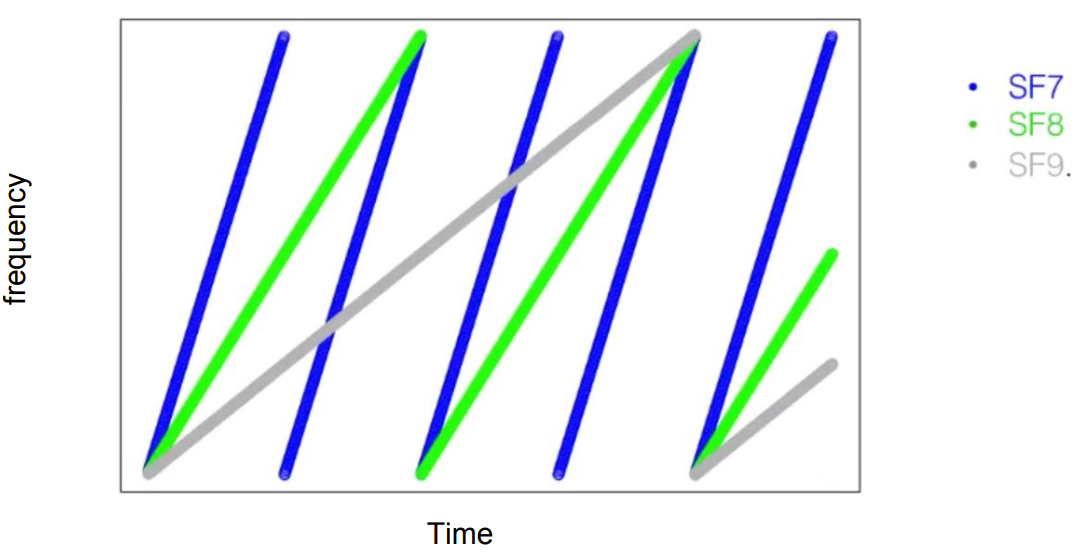
\includegraphics[width=0.5\textwidth]{Figures/spreading factors.png}
	\caption{Chirp signál a porovnanie spreading factoru. Prevzaté z \cite{spreadfactorimage}}
	\label{fig:spreadingfactors}
\end{figure}

Chirp signál je rozdelený na X častí -- tzv. chips. Tieto chips predstavujú skoky vo vysielacej frekvencii signálu. 
Koľko týchto chips jeden chirp obsahuje je závisle od vybraného spreading factoru. 
Jeden chirp je rozdelený na $2^{SF}$ častí alebo chips. Vysielaný symbol sa potom skladá z cyklicky posunutého chirp signálu, kde posun definuje hodnotu daného symbolu. 
To znamená, že vysielaný chirp nebude začínať na spodnej hranici frekvenčného pásma, ale na určitej frekvencii korešpondujúcej so symbolom, 
ktorý je modulovaný do daného chirpu. Viď Obr. \ref{fig:loraSymbols}.

\begin{figure}
	\centering
	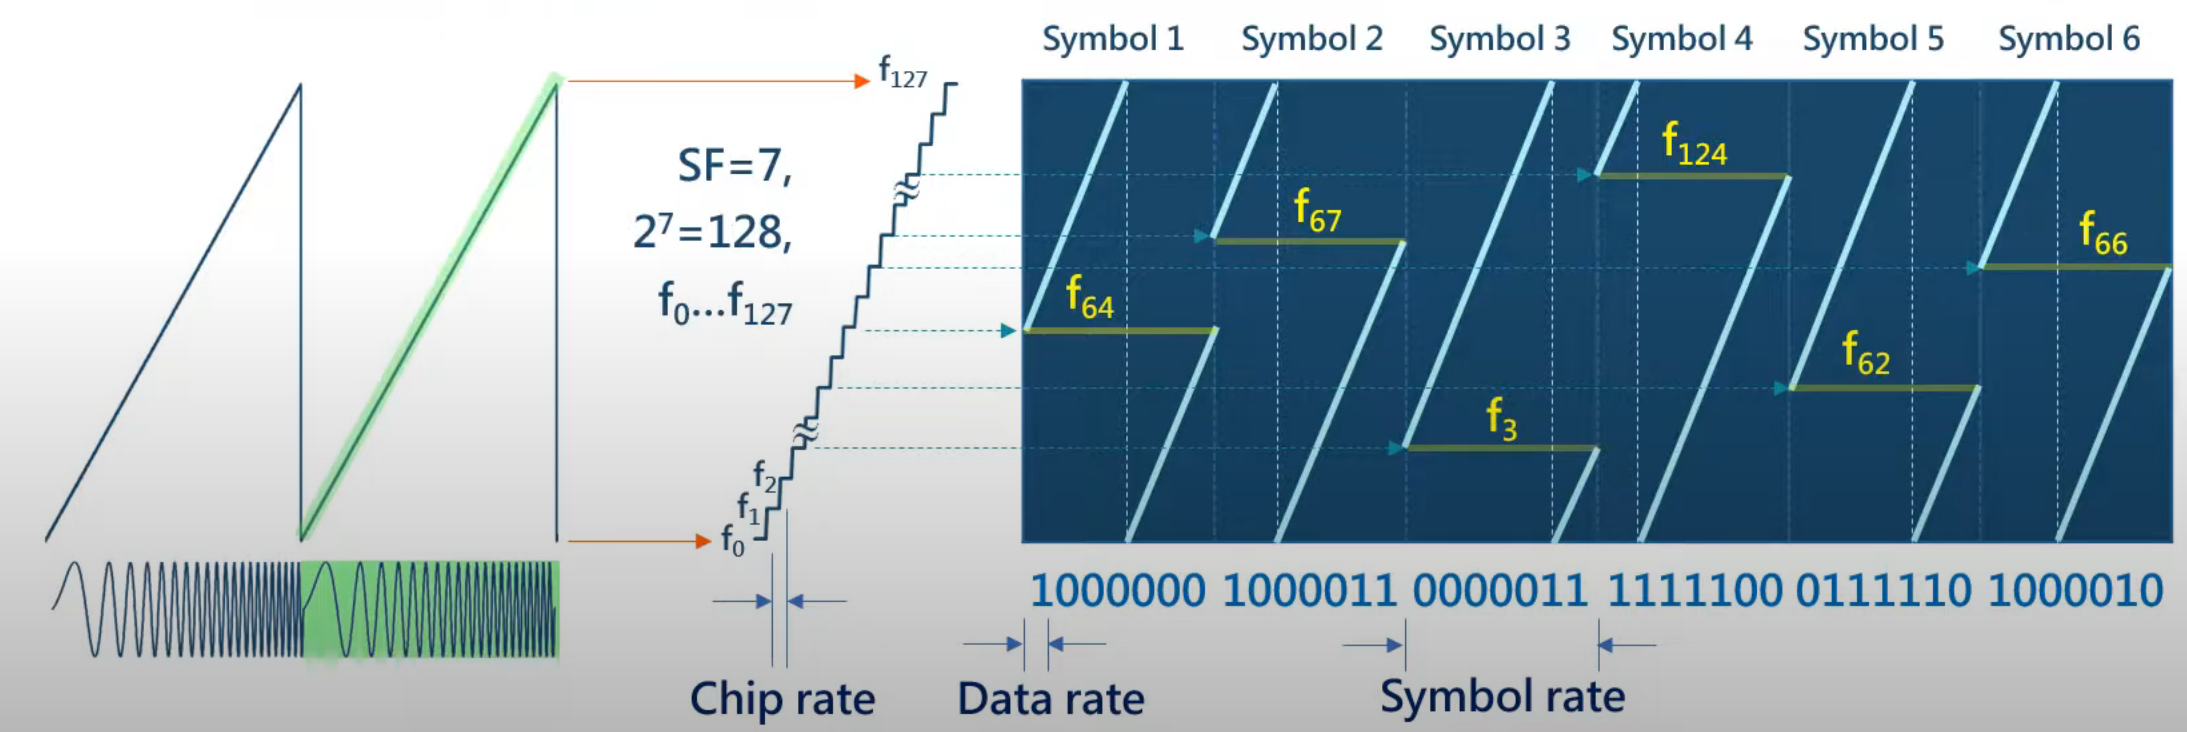
\includegraphics[width=1\textwidth]{Figures/loraSymbols.png}
	\caption{Chirp signály, do ktorých boli modulované symboly. Prevzaté z TODO}
	\label{fig:loraSymbols}
\end{figure}

Celý proces vyslania správy cez LoRa sa teda skladá z nasledujúcich krokov:
\begin{enumerate}
  \item Konverzia správy do binárneho kódu
  \item Pridanie korekčných bitov slúžiacich na opravu chýb
  \item Pridanie preambuly a kontrolného súčtu, a poskladanie do LoRa packetu
  \item Modulacia bitov do chirp signálov
  \item Odvysielanie chirp signálov
\end{enumerate}
Ukážku môžme vidieť na Obr. \ref{fig:loraModulation}.

\begin{figure}
	\centering
	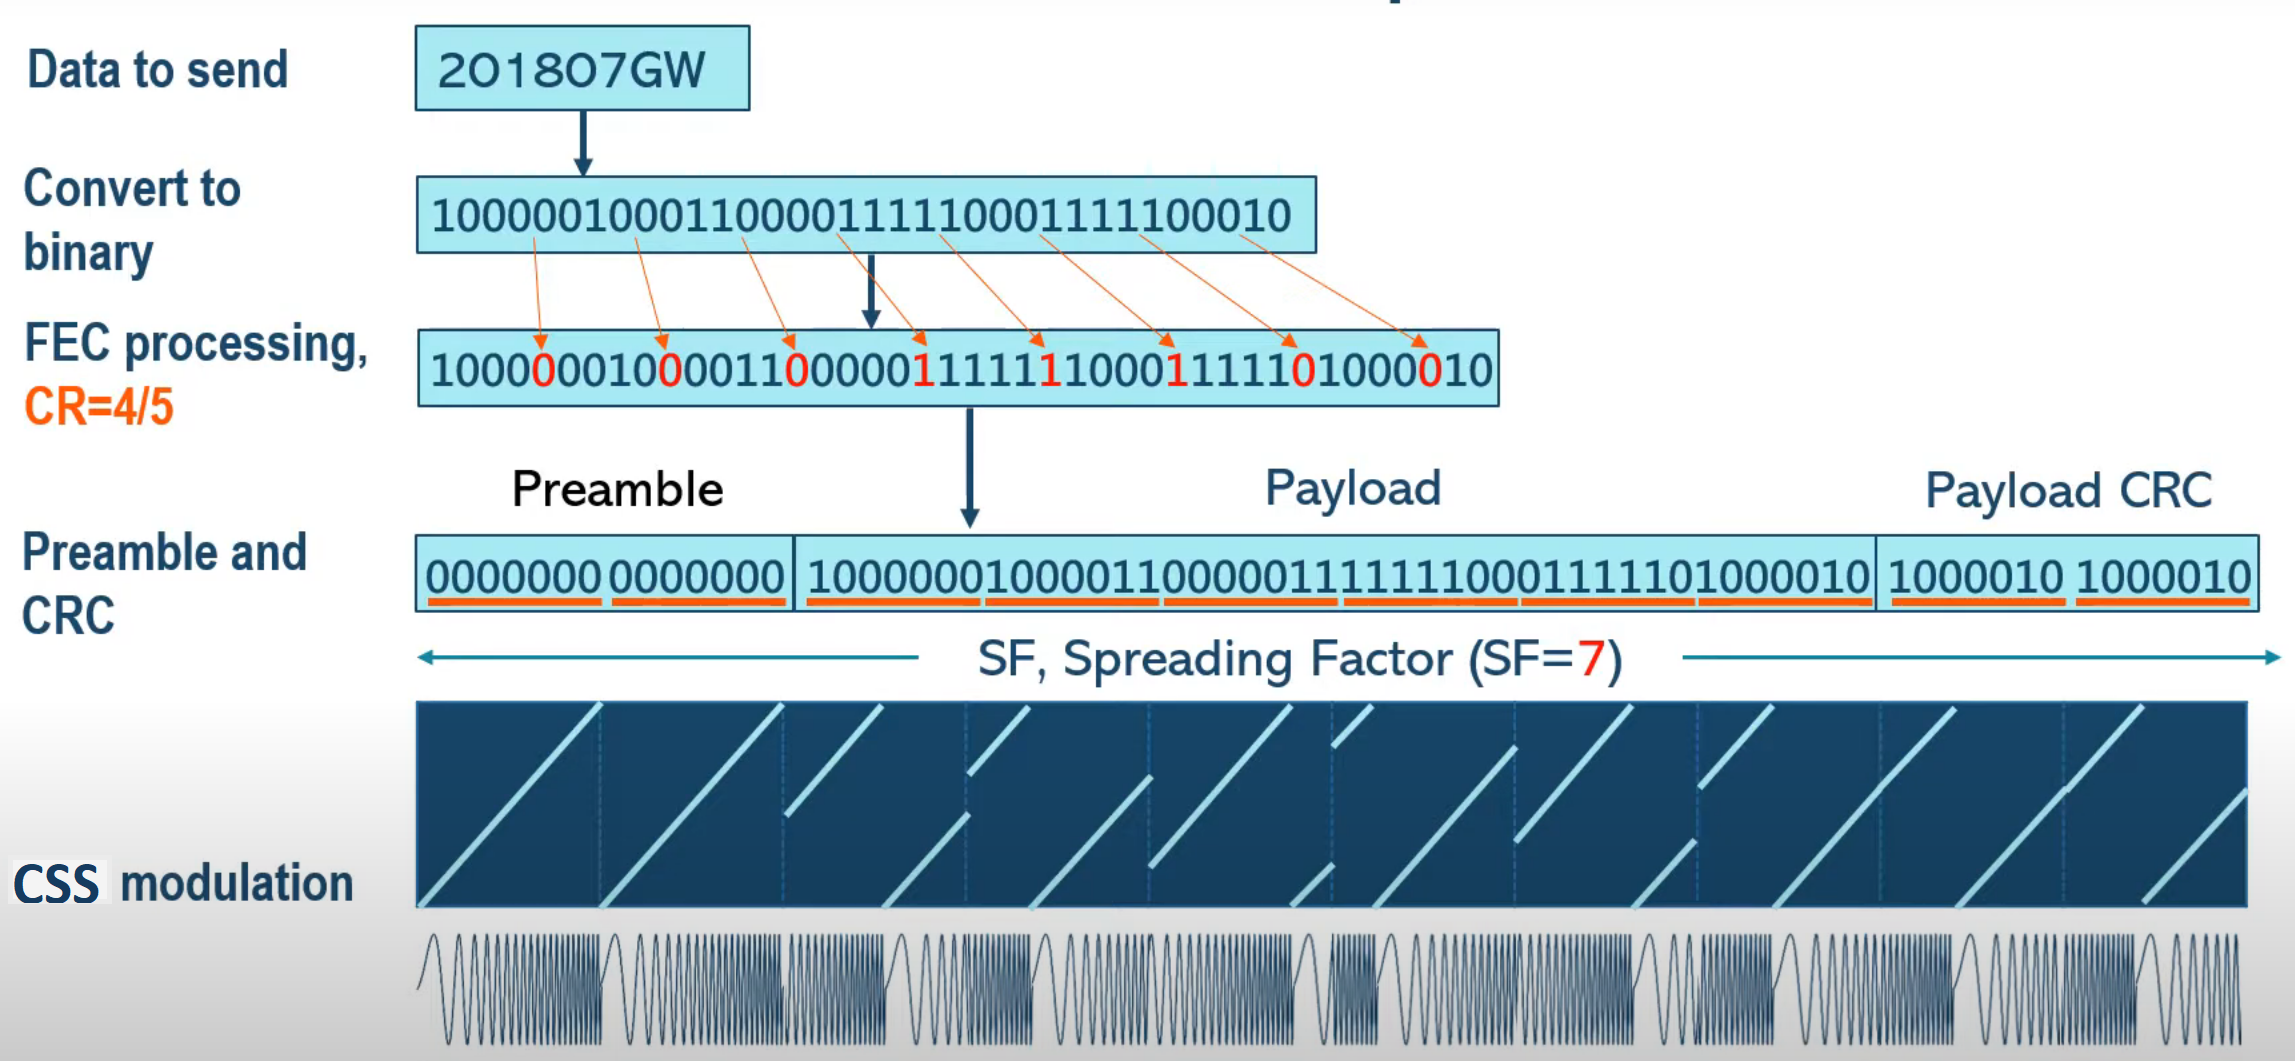
\includegraphics[width=1\textwidth]{Figures/loraModulation2.png}
	\caption{Proces spracovania odosielaných dát v LoRa (Binárne hodnoty su vymyslené, nezodpovedajú reálnej konverzií). Prevzaté z TODO}
	\label{fig:loraModulation}
\end{figure}

\section{LoRa packet}
Štruktúra LoRa packetu môže byť závisla od daného použitia. Bežné sa ale stretávame s LoRa packetom 
, zloženým z preambuly, dát a kontrolného súčtu.

Preambula slúži na synchronizáciu prijímacieho zariadenia. Je tvorená X opakovaniami prázdneho chirp signálu.
Dĺžka preambuly, tzn. počet opakovaní prázdneho chirp signálu, je stanovená konfiguráciou zariadenia. Bežne je používana dĺžka preambuly 8.
Na Obr. \ref{fig:loraModulation} môžme vidieť, že na preambulu boli použité iba 2 prázdne chirp signály -- teda dĺžka preambuly je 2.

Prijímacie zariadenie číta prijaté symboly v určitom časovom intervale. Tento interval sa ale nemusí zhodovať s intervalom, ktorý bol použitý pri vysielaní daných symbolov.
Je preto potreba synchronizovať prijímacie zariadenie aby hodnoty symbolov boli správne interpretované.

Zariadenie po prijatí nového packetu očakáva, že na začiatku bude preambula definovanej dĺžky. Ak z packetu prečíta počet symbolov rovnakej hodnoty, zhodný 
s definovanou dĺžkou preambuly, vie že sa jedná o preambulu a synchronizuje čítacie okno tak aby bolo zarovnané so symbolmi preambuly. Tzn. tak, aby symboly preambuly boli 
symbol 0. Zjednodušené znázornenie procesu čítania symbolov a posun čítacieho okna môžme vidieť na Obr. \ref{fig:loraPreamble1}.

\begin{figure}[h!]
	\centering
	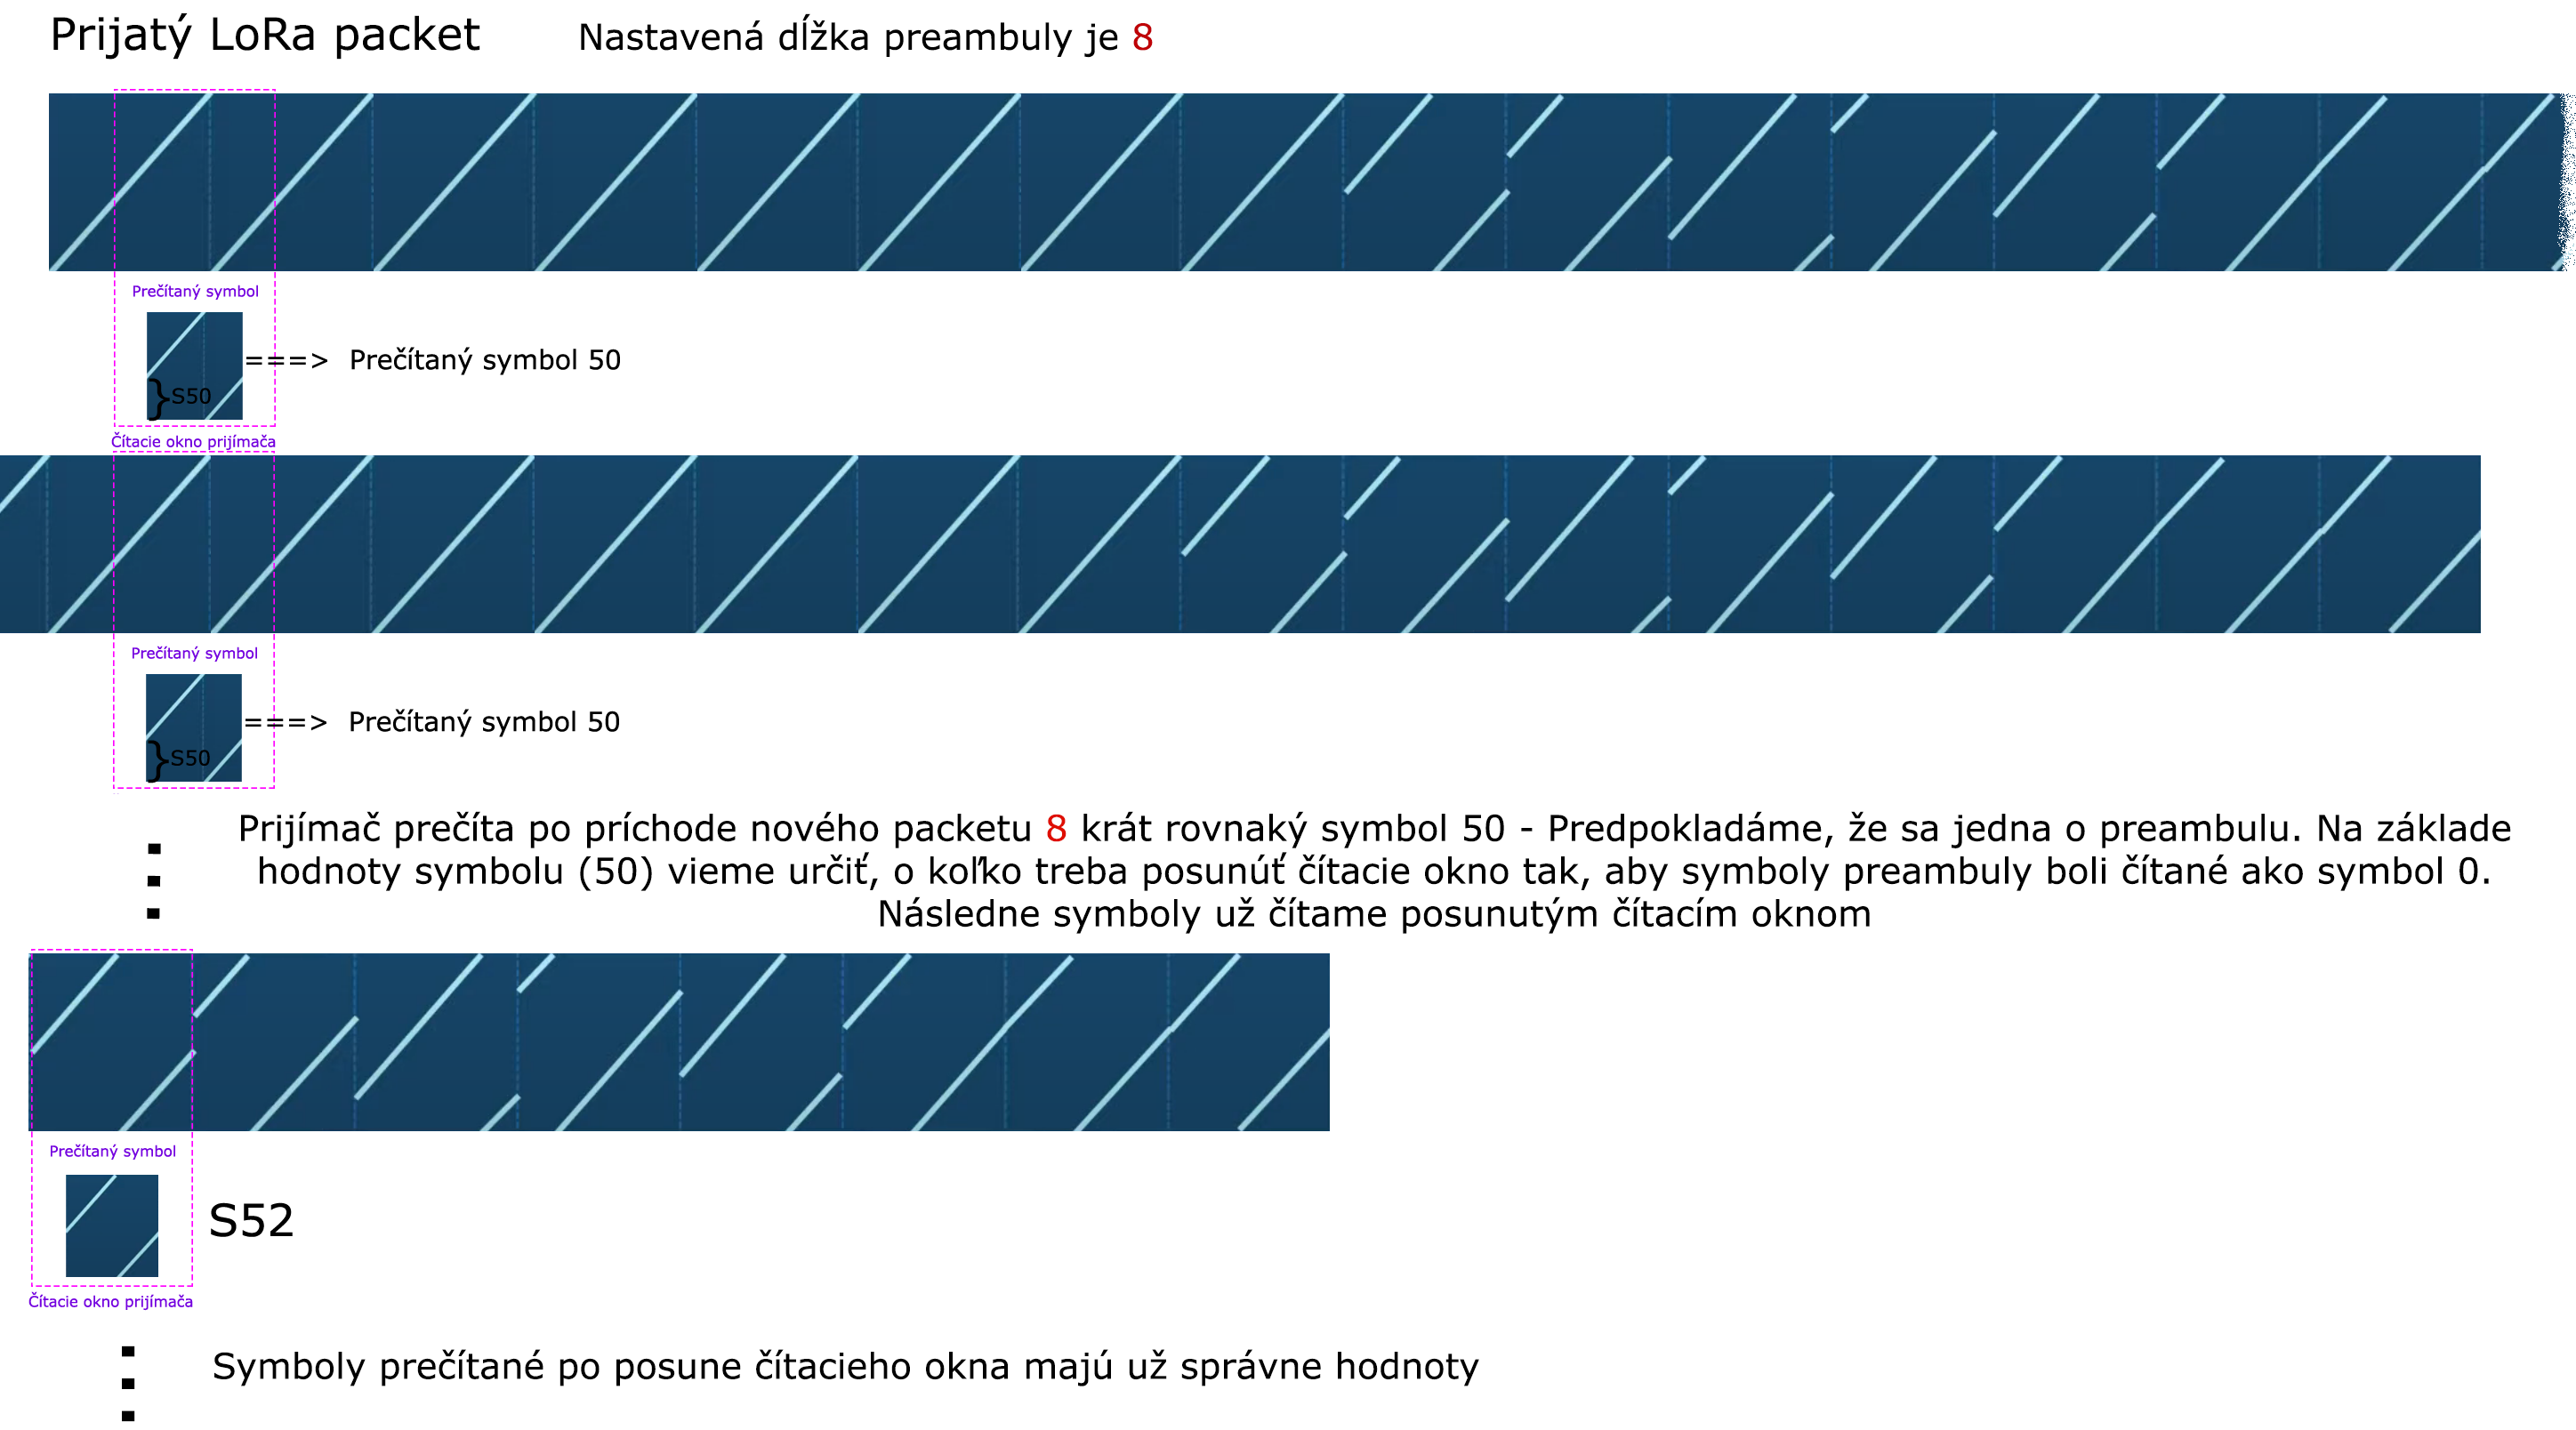
\includegraphics[width=1\textwidth]{Figures/preambulaSmall.png}
	\caption{Čítanie symbolov preambuly prijatého packetu a synchronizácia čítacieho okna na základe posunu preambuly.}
	\label{fig:loraPreamble1}
\end{figure}

\newpage
\section{LoRa parametre}
Pri používaní LoRa je nutné správne zvoliť parametre prenosu. Sú nimi frekvencia, bandwidth, spreading factor a coding rate.
Použitá frekvencia je závisla od regiónu, v ktorom sa používa, viď Tabuľka \ref{tab:ismBands}. 
V Európe je možné mimo 866 MHz pásma používať aj 433 MHz pásmo. Okrem toho existuje ešte globálne používaná frekvencia 2,4 GHz.

\begin{table}[h!]
	\centering
  \small
  \setlength\tabcolsep{6pt}
	\caption[Frekvenčne pásma používane pre LoRa]{Frekvenčne pásma používane pre LoRa}
  \begin{tabular}{c|c}
    \toprule
    Region & Frekvencia (MHz)\\
    \midrule
    Ázia & 433 \\
    Európa, Rusko, India, Afrika & 863--870 \\
    Severná Amerika & 902--928 \\
    Austrália & 915--928 \\
    Kanada & 779--787 \\
    Čína & 779--787, 470--510 \\
    \midrule
  \end{tabular}
  \label{tab:ismBands}
\end{table}


Ostatné parametre sú vyberané na základe toho ako ďaleko, ako spoľahlivo a ako rýchlo je potrebné dáta prenášať. Je nutné zvoliť vhodný kompromis medzi rýchlosťou prenosu 
a dosahom prenosu.

Parameter bandwidth určuje šírku pásma, v ktorom sa bude chirp posúvať. Pri vyššom bandwidthe sa zvyšuje rýchlosť prenosu, avšak znižuje sa použitelný dosah.

Spreading factor určuje koľko bitov dát bude prenesených v každom vysielanom symbole. To určuje ako rýchlo sa chirp posúva po frekvenčnom pásme a tym pádom 
zvyšuje alebo znižuje rýchlosť prenosu na úkor zniženia alebo zvýšenia dosahu prenosu. Spreading factor je vo väčšine prípadov možné zvoliť z intervalu 6--12. 
Avšak niektoré LoRa moduly umožnujú nastavit aj nižšie hodnoty. 
%TODO ortogonalita spravne slovo ?
Používanie spreading factorov prináša výhodu v podobe ortogonality sprav. To znamená, že prijímač dokáže správne prijať a dekódovať správu poslanú so spreading factorom X aj 
keď sa vysielaná správa časovo prekrýva s inou vysielanou správou s iným spreading factorom.

LoRa obsahuje korekciu chýb spôsobených rušením. Využíva k tomu samoopravný kód -- forward error correction, pri ktorom 
sa ku prenášaným dátam pridavajú korekčné bity. Tieto bity sú potom na prijímacej strane použité na detekciu a prípadnu opravu chyby ak k nejakej došlo.
K nastaveniu korekcie chýb slúži parameter coding rate.
%TODO preformulovat pomer, realne je to pomer bitov ktore nesu informaciu ku bitom ktore nesu uinformaciu + opravne bity (4/5 => 4 + 1 opravny bit == 5)
V LoRa máme na výber zo štyroch možností coding rate: 4/5, 4/6, 4/7 a 4/8. Označenie vyjadruje pomer bitov, ktoré nesú informáciu, ku bitom, ktoré sú 
použité na korekciu chýb. Napríklad pri coding rate 4/5 sa na každé 4 bity informácie pridáva 1 korekčný bit.
Vyšší coding rate zabezpečí spolahlivejší prenos ak sa nachádzame v rušivom prostredí, ale zníži rýchlosť prenosu dát, 
pretože ku prenášaným dátam pridáva navyše dáta potrebné na korekciu chýb.

Rýchlosť prenosu dát (Data rate -- DR) v kbps môžme vyjadriť vzťahom:
\begin{equation}
  DR = SF * \frac{BW}{2^{SF}} * \frac{4}{4+CR}
\end{equation}

\section{LoRaWAN}
LoRa je definovaná len na fyzickej vrstve. Na používanie LoRa v IoT sieťach sú však potrebné aj vyššie vrstvy sieťového modelu.
K tomu vznikol protokol LoRaWAN, ktorý je spravovaný organizáciou LoRa Alliance \cite{lora}.

LoRaWAN definuje komunikačný protokol a architektúru sieti. Siete používaju hviezdicovú alebo hviezdu hviezd topológiu, kde 
centrálnym uzlom je LoRaWAN gateway, ktorý je pripojený k internetu. Ostatne uzly siete posielajú dáta na gateway, ktorá ich preposiela na internet.

LoRaWAN definuje tri triedy zariadení, ktoré sa v sieti vyskytujú. Sú nimi triedy A, B a C, kde do triedy A spadajú zariadenia 
väčšinou poháňané batériami, ktoré po odvysielaní svojích dát otvarajú dve prijímacie okna, v ktorých čakajú na príjem dát z gateway.
Trieda B je rozšírením triedy A. Zariadenia v tejto triede môžu otvárať dodatočné prijímacie okna v naplánovaných časových intervaloch.
Zariadenia z triedy C môžu prijímať neustále. Z tohto dôvodu majú vyššiu spotrebu energie a zvyčajne su pripojené k stálemu napájaniu.
%TODO trosku viacej nech nieje prazdna skoro cela strana pred dalsiou kapitolou

\section{Legislativa}
V Európe sa k frekvenčnému pásmu používaného pre LoRa viažu určité obmedzenia. 
Obmedzenia sa týkaju používania fyzického média. Regulácia určuje maximálnu povolenú dobu, v ktorú môže vysielač na daných frekvenciach vysielať 
v rámci jednej hodiny a maximálny vysielací výkon, akým môžme signal vysielať.
Určuje sa klučovací pomer, ktorý hovorí koľko percent času z nejakého celkového času môže vysielač vysielať.

Ak by zariadenie vysielalo signál po dobu jednej jednotky času z celkových 10 jednotiek času, tak kľučovací pomer by bol 10 \%.

Český Telekomunikačný úrad \cite{ctu} stanovuje vo všeobecné oprávnění č. VO-R/10/07.2021-8 \cite{vor}, že 
frekvenčné pásmo, do ktorého spadá LoRa, patrí do skupiny g. Pre túto skupinu je maximálny povolený kľučovací pomer 1 \% a maximálny 
vysielací výkon 25 mW (14 dBm). Znamená to teda, že zariadenia môžu každú hodinu vysielať maximálne po dobu 36 sekúnd.
Pre pásmo 869,40--869,65 MHz je ale udelená výnimka, ktorá umožňuje vysielať s kľučovacím pomerom 10 \% a maximálnym vysielacím výkonom 500 mW (27 dBm).


\chapter{Dostupné LoRa moduly }
Pri práci s LoRa technológiou máme na výber z rôznych modulov od rôznych výrobcov.
Moduly môžme rozdeliť podla použitia na moduly pre koncové zariadenia a moduly pre gateway.
Moduly pre koncové zariadenia obvykle dokážu prijímať a odosielať iba na jednom kanále ( kombinácia LoRa parametrov --  BW, SF a frekvencia ) súčasne a majú 
nízku spotrebu energie. Moduly pre gateway dokážu prijímať a odosielať na viacerých kanáloch súčasne a majú vyššiu spotrebu energie.

V tejto časti sa budeme zaoberať dostupnými modulmi pre koncové zariadenia.
Kedže je technológia LoRa patentovaná výrobcom Semtech \cite{semtech}, tak všetky dostupné LoRa chipy su od tohto výrobcu a moduly od iných výrobcov 
sú založené na používani týchto chipov.

\section{SX127x/SX126x}
Výrobca Semtech \cite{semtech}, prináša LoRa chipy série SX127x a SX126x. Ponukajú vysoký výkon za pomerne nízku cenu a ako sme už spomínali, ostatné LoRa moduly 
implementuju tieto chipy -- modemy a rozširujú ich o ďalšiu funkcionalitu.

\subsection{SX127x}

SX127x LoRa modemy používajú frequency hopping spread-spectrum moduláciu. Čo znamená, že viaceré vysielané signály môžu zaberať rovnaký kanál, ktorý ma vysokú ochranu proti rušeniu a zároveň majú nízku spotrebu energie. %TODO divna veta ??

Modemy používajú LoRa modulačnú techniku, patentovanú firmou Semtech. Maximálny vysielací výkon modemov je 100 mW.
Vďaka tejto modulačnej technike je možné dosiahnúť vysokej citlivosti modemov.
Výrobca uvádza citlivosť cez -137 dBm pri modemoch SX1272/73 a -148 dBm pri modemoch SX1276/78/79.

Modemy SX1272 a SX1273 ponukajú menší link budget 157 dB oproti 168 dB pri modemoch SX1276/77/78/79 a majú menší rozsah frekvenčných pásiem medzi 860 a 1020 MHz.
Okrem toho majú aj vyššiu spotrebu energie.

Pri modemoch SX1276/77/78/79 je možné vybrať frekvenčné pásma z rozsahu 137 až 1020 MHz.

\subsection{SX126x}

Modemy zo série SX126x - SX1261/62/68 sú následovníkmi modemov SX127x. Majú väčší vysielací výkon vďaka integrovanému zosilovaču a menšiu spotrebu energie. Obsahujú precízny TCXO oscilátor, 
ktorý zabezpečuje presnejšie a stabilnejšie riadenie počas prevádzky modemu. Okrem LoRa modulácie obsahujú aj G(FSK) moduláciu, ktorá je vhodná pre staršie 
prípady užitia.

Modemy taktiež obsahujú +22/+15 dBm zosilovač, vďaka ktorému majú vyšší link budget oproti modemom zo série SX127x -- 170 dBm,
takže sú optimálne pre aplikácie vyžadujúce väčší dosah alebo robustnosť.
%TODO tu sa trochu este rozpisat viac... co je link budget napr atd. este modem 1280/1281 - 2.4ghz

\begin{table}[!h]
	\centering
  \small
  \setlength\tabcolsep{6pt}
	\caption[Parametre Semtech modemov]{Parametre Semtech modemov}
  \begin{tabular}{c|c|c|c|c|c|c|c|c}
    \toprule
    Modem & Frekvencia & SF & BW (kHz) & Citlivosť & Spotreba \footnotemark[0] & Rozhranie & Výkon\footnotemark[1] & Cena\footnotemark[2]\\
    \midrule
    SX1272 & 860--1020 MHz & 6--12 & 125--500 & -137 dBm & 11,2 mA & SPI & 20 dbm & 9€ \\
    SX1273 & 860--1020 MHz & 6--9 & 125--500 & -130 dBm & 11,2 mA & SPI & 20 dbm & 7€ \\
    SX1276 & 137--1020 MHz & 6--12 & 7,8--500 & -148 dBm & 12 mA & SPI & 20 dbm & 10€ \\
    SX1277 & 137--1020 MHz & 6--9 & 7,8--500 & -139 dBm & 12 mA & SPI & 20 dbm & 7€ \\
    SX1278 & 137--525 MHz & 6--12 & 7,8--500 & -148 dBm & 12 mA & SPI & 20 dbm & 8€ \\
    SX1279 & 137--960 MHz & 6--12 & 7,8--500 & -148 dBm & 12 mA & SPI, UART & 20 dbm & 11€ \\
    \hline
    SX1261 & 150--690 MHz & 5--12 & 7,80--500 & -125 dBm & 8 mA & SPI & 15 dbm & 7€ \\
    SX1262 & 150--690 MHz & 5--12 & 7,80--500 & -125 dBm & 8 mA & SPI & 22 dbm & 8€ \\
    SX1268 & 410--810 MHz & 5--12 & 7,80--500 & -148 dBm & 4.6 mA & SPI & 22 dbm & 7€ \\
    \midrule
  \end{tabular}
\end{table}
\footnotetext[0]{Spotreba počas prijímania (mA)}
\footnotetext[1]{Maximálny vysielací výkon}
\footnotetext[2]{Cena platná ku Q4 2022}

\section{RFM9xW}
Moduly RFM95W/96W/98W od výrobcu HopeRF \cite{hoperf} implementujú SX LoRa modemy od výrobcu Semtech.
Jedná sa o jednoduchý modul, ktorý obsahuje všetku riadiaciu elektroniku potrebnú na riadenie Semtech LoRa modemu.
Okrem riadiacej elektroniky obsahuje modul aj zosilovač signálu (+14 dBm), ktorý zvyšuje dosah bezdrôtového prenosu.

Existuje niekoľko verzií modulov RFM9xW, kde každá verzia používa iný semtech LoRa modem a zdiela parametre daného modemu.

\section{Moduly a zariadenia použité v tejto práci}
Na vývoj a testovanie tejto práce boli použité rôzne zariadenia s rôznymi platformami. Na simulovanie jednoduchých koncových zariadení, 
ktoré môžu predstavovať napríklad nejaký senzor, boli použité mikrokontroléry TTGO od výrobcu LILYGO \cite{lilygo}.

Okrem mikrokontrolérov TTGO boli použité aj mikrokontroléry Raspberry Pi Pico a mikropočítáč Raspberry Pi.
Všetky mikrokontroléry môžu byť rozšírene o batériu a byť mobilné.
%TODO obrazky ttgo modulov?

\subsection{TTGO LoRa32}
Mikrokontrolér založený na module ESP32. Obsahuje Wi-Fi a bluetooth. Používa SX1276 LoRa modem.
Dá sa prepnúť do úsporného režimu, ktorý znižuje spotrebu mikrokontroléru na 0,6 mA.
Mikrokontrolér obsahuje aj display, ktorý je pripojený cez I2C rozhranie.

\subsection{TTGO T-Beam}
Tento mikrokontrolér je taktiež založený na module ESP32 a používa SX1276 LoRa modem. Okrem Wi-Fi a bluetooth obsahuje aj GPS modul.
V režime spánku ma spotrebu 0,2 mA.

\subsection{Raspberry Pi Pico}
Mikrokontrolér založený na dvoj-jadrovom Arm procesore. Existuje verzia s Wi-Fi modulom. Na programovanie sa využíva microPython. %TODO ref na microputhon?
V tejto práci boli mikrokontroléry použité spolu s RFM96W modulmi pre prácu s LoRa.

\subsection{Raspberry Pi 3?4? TODO}
Na rozdiel od predchádzajúcich mikrokontrolérov má tento mikropočítáč ovela väčši výkon a pamäť. Z toho dôvodu bude na tomto zariadeni pridaná 
možnosť monitorovania a zachytavania správ v LoRa sieti. Zariadenie obsahuje ethernetový port, ktorý môže slúžiť na pevné pripojenie do internetovej siete.
Pre prácu s LoRa bude použitý RFM96W modul.


\chapter{Existujúce riešenia}
Téma mesh sietí je v tejto dobe velmi aktuálna a vývojári sa snažia vytvoriť rôzne riešenia, ktoré by boli vhodné pre rôzne účely.
Existujú rozvinuté projekty ako napríklad Meshtastic, ktorý sa snaží vytvoriť rozsiahlu decentralizovanú mesh sieť za použitia lacných zariadení.

Ďalším zaujímavým projektom je Armachat \cite{armachat}, ktorý ponúka možnosť komunikácie v prípade nedostupnosti ostatných sieti, napríklad po nejakej prírodnej alebo inej katastrofe.
Súčastou projektu Armachat sú dostupné návhry plošných spojov, ktoré implementujú Raspbery Pi Pico mikrokontroléry, RFMx LoRa moduly, display a ďalšie vymoženosti.
Výsledkom poskladania týchto plošných spojov je malé mobilné zariadenie s klávesnicou a displejom, ktoré sa dá použiť na komunikáciu prostredníctvom LoRa siete.
Originálny projekt avšak plne nepodporuje využívanie mesh topologie. Používa ale rovnakú štruktúru správ ako projekt Meshtastic a vďaka tomu je možné 
v Armachate využívať mesh sieť projektu Meshtasticu.

\section{Lora mesher}
LoRaMesher \cite{loramesher} je knižnica, ktorú je možné použiť na komunikáciu cez LoRa mesh sieť.

Na smerovanie v sieti sa používa distance vector routing protocol. Tento protokol vyberá cestu, kadiaľ pôjde správa od odosielateľa k príjemcovi, na základe 
najlepšej cesty. Najlepšiu cestu definuje ako cestu s najmenším počtom hopov -- preskokov medzi uzlami v mesh sieti.

K realizacií distance vector smerovania je potrebné mať smerovaciu tabuľku, ktorá obsahuje informácie o ID uzlov, cez ktoré susedné uzly sa dajú dosiahnuť a 
koľko preskokov bude potrebných na dosiahnutie týchto uzlov. Smerovacia tabuľka je periodicky aktualizovaná cez špeciálny typ správ, ktoré sú odosielané 
všetkými uzlami v sieti. Túto smerovaciu tabuľku si drží každý uzol v sieti.

LoRaMesher používa FreeRTOS, čož je operačný systém reálneho času. Takéto operačné systémy garantujú dokončenie úloh v určitom čase.
FreeRTOS je použitý na zabezpečenie plánovania úloh. Rozličné úlohy sa starajú o prijatie a odoslanie packetov, iné úlohy sa starajú o samotne 
spracovanie prijatých packetov.

LoRaMesher dokáže nájsť novo vytvorené uzly v sieti vďaka smerovaciemu protokolu. Pri odoslaní správ čaká na prijatie ACK správy, ktorá potvrdzuje, 
že správa bola prijatá a tým zaistuje spoľahlivosť. Správy väčšie ako 222 bajtov rozdeluje na viacero správ, ktore pošle postupne.

\section{Meshtastic}
Meshtastic \cite{meshtastic} vytvára mesh sieť za použitia lacných mikrokontrolérov s LoRa modulmi.
Myšlienka tohto projektu spočíva v tom, že vytvára komunikačnú sieť na miestach kde neexistuje spoľahlivá infraštruktúra na bezdrôtovú komunikáciu (napr. v horách).

Posielanie správ v sieti je založené na jednoduchom multi-hop floodingu.
Každý uzol znovu odvysiela packet, ktorý prijal ( pokial nedošiel počet preskokov na 0 ), až kým sa packet nedostane do určenej destinácie naprieč mesh sietou.
Prenášane správy su šifrované.

Používane zariadenia s LoRa modulmi majú zabudovaný bluetooth chip, vďaka ktorému je možne sa k zariadeniu pripojit cez smartphone, ktorý slúži ako rozhranie pre 
užívateľa. Cez aplikáciu v smartphone môže používateľ vytvárať a prijímať správy. Správy sa cez bluetooth prenášaju zo smartphone do zariadenia a odošlu sa cez 
LoRa do siete. %TODO trosku preformulovat

Meshtastic poskytuje možnosť pripojenia sa k oficiálnemu meshtastic mqtt brokerovi. Toto umožňuje prepojiť malé lokálne mesh siete do väčšej globálnej siete a 
tak rozšíriť dosah siete.

\section{LoRaBlink}
Multi-hop protokol, ktorý požíva časovú synchronizáciu medzi uzlami. Časová synchronizácia definuje sloty, v ktorých môže uzol pristupovať ku prenosovému médiu a 
vysielať svojé dáta. Správy sa sieťou šíria pomocou multi-hop floodingu.

Sieť sa skladá z jedneho datasinku (gateway) a viacerých uzlov. Uzly sieťe posielajú data do datasinku alebo data z neho prijímaju.
V určitých intervaloch datasink vyšle tzv. beacon signál. Tento signál slúži na časovú synchronizáciu medzi uzlami a znači začiatok novej epochy. 
Každá epocha obsahuje N slotov, v ktorých môžu uzly vysielať data. Beacon správa obsahuje hop count, ktorá udáva vzdialenosť ku datasinku.
Ked nejaký uzol príjme beacon signál, vyšle svoj vlastný beacon signál v dalšiom volnom slote, ktorý vyberá na základe vzdialenosti od datasinku (hop count).

Ked uzol potrebuje poslať nejaké data, tak vyberie najskorší volný slot a v nom vysiela data. Ak tieto data príjme uzol, ktorý nieje datasink a 
hop count daného uzlu ku sinku je menší ako hop count vysielajucého uzlu, tak data v dalšiom slote znovu prepošle. Toto sa opakuje, až 
kým data nedosiahnu datasink.
%TODO dostudovat, rozsirit popis

Takto tvorená sieť avšak vyžaduje existenciu nejakého hlavného uzlu (datasinku), ktorý je potrebný na riadenie siete prostredníctvom časovej synchronizácie.

\section{Pymesh}
Pymesh je súčasťou Pycom \cite{pycom} ekosystému. Tento ekosystém je určený na vývoj IoT systémov. Ponúka rôzne zariadenia, ktoré su určené na použitie s týmto 
ekosystémom. Zariadenia WiFi, bluetooth a LoRa. Zariadenia je možné rozšíriť o rôzne moduly so senzormi, ktoré rozšírujú ich schopnosti. %TODO preformulovat

PyMesh sieť sa skladá z uzlov, ktoré môžu vystupovať v roli gateway alebo bežného uzla. Uzly typu gateway su označované ako Border Routers a prepájajú LoRa sieť s 
internetom. Uzly v sieti môžu komunikovať ad-hoc. V sieti môže dojsť k situacií kedy bude chcieť viacero uzlov vysielať v rovnakom čase a došlo by tak ku kolizií.
Aby sa zabránilo takýmto situáciam, je použitá metóda Listen Before Talk, pri ktorej sa pred vysielaním signálu overí, či nie je v sieti už niekto iný, kto by 
vysielal. Pokial je, tak sa signál vyšle neskôr.

PyMesh je primárne určený na použitie s Pycom zariadeniami a použitie na inom zariadení by vyžadovalo väčšie úpravy zdrojového kódu.

\section{Synchronous LoRa Mesh}
Tento projekt\cite{synchronouslorameshnetwork} vznikol z potreby získavania real-time dát z podzemných kanalizácií. Tieto dáta sú potrebné k monitorovaniu a predikcií kritických situacií akými 
sú napríklad záplavy.

LoRaWan však nema moc velký dosah do podzemia. Z toho dôvodu by bolo potrebné v podzemných priestoroch implementovať LoRaWan gateway-e, ktoré su ale energeticky náročne, drahé a vyžadujú 
pevné pripojenie do elektrickej a prípadne aj internetovej siete. Okrem toho, by museli byť všetky ostatné uzly v podzemnej sieti v dosahu gateway a pri väčšej podzemnej sieti 
by teda bolo potrebné implementovať viacero LoRaWan gateway.

Tento projekt sa snaží vyriešiť tieto problémy. Prináša protokol, ktorý rozširuje LoRaWan o tzv. repeater uzly (RN) viď Obr. \ref{fig:synchronouslora}. Tieto uzly sa vyskytujú na povrchu a preposielajú dáta z 
podzemných monitorovacích uzlov (sensor node  - SN) do LoRaWan siete. Monitorovacie uzly pod zemou tvoria mesh sieť a RN plní funkciu riadiaceho uzlu pre podzemnú mesh siet. 
Komunikácia medzi RN a SN je synchronizovaná pomocou presného časovania, čo umožňuje koordináciu zmeny stavov SN z režimu spánku do normálneho režimu v čase, kedy 
potrebuje SN prijímať a odosielať dáta. Komunikácia sa cez uzly šíri multi-hop prístupom, za použitia smerovacej tabulky.

Protokol používa na riadenie komunikácie metódu TDMA. RN priradí každej SN časový slot, v ktorom SN môže vyslať alebo prijať dáta.
Monitorovacie uzly su väčšinu času v režime spánku, zobudia sa len v ich určenom časovom slote a vďaka tomu maju tieto uzly nízku spotrebu energie.

Novo pripojený uzol do sieťe musí čakať na periodicky beacon, vysielaný RN uzlom. Všetky uzly si držia v sebe smerovaciu tabuľku. Po pripojení nového uzla sa sieťou sa propaguje 
správa na aktualizovanie smerovacej tabuľky.

\begin{figure}
	\centering
	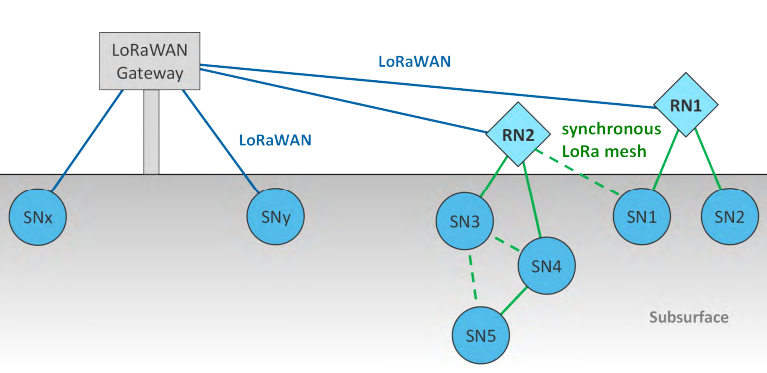
\includegraphics[width=0.6\textwidth]{Figures/synchronouslorameshnetwork.png}
	\caption{Schéma Synchronous Lora Mesh. Prevzaté z \cite{synchronouslorameshnetwork}}
	\label{fig:synchronouslora}
\end{figure}

\section{Porovnanie voči nášmu riešeniu}
Niektoré zo spomenutých riešení využívaju smerovacie tabuľky na efektívnejši prenos dát v rámci siete. Smerovacie tabuľky môžu byť však limitáciou pokiaľ 
chceme dosiahnuť mobility uzlov. V tom prípade je potrebné zabezpečiť dostatočne časté aktualizácie smerovacích tabuliek.

Niektoré spomenuté riešenia limitujú komunikáciu medzi uzlami na vyhradené časové okná, mimo ktoré su uzly v úspornom režime. To môže byť 
veľkou limitacou pri niektorých aplikáciách, kde je potrebná komunikácia v reálnom čase  (napr. chat).

Protokol navrhnutý v tejto práci nebude využívať žiadne smerovacie tabuľky. Vďaka tomu dosiahneme mobility uzlov bez potreby 
periodických aktualizacií smerovacích tabuliek. Protokol nebude používať žiadnu časovú synchronizáciu ani časové okná vyhradené na komunikáciu, 
uzly siete tak budu môcť prijímať a odosielať dáta hocikedy.

Funckionalita navrhnutého protokolu bude podobná ako projekt Meshtastic, kedy sa správa v sieti preposiela až kým nedorazí do destinácie.
Správa sa odošle a uzol, ktorý túto správu prijal ako posledný ju prepošle dalej. Toto sa opakuje na dalších uzloch až kým sa správa nedostane do destinácie alebo kym správe nedôjde hoplimit.

Ak nieje destinácia v dosahu, tak o správu prídeme. Tento problém vyriešime tak, že odosielatel si bude odoslané správy ukladať a v prípade, že sa nepodarí správu doručiť, môže ju opätovne 
odoslať niekedy neskôr.

Navrhnutý protokol nieje závisly na žiadnych špeciálnych uzloch typu gateway, prípadne riadiacich uzloch. Každý uzol v sieti môže byť primitivným uzlom, ktorý bude prijímať a preposielať dáta.
Vďaka tomu môžu byť uzly realizované prostredníctvom lacných a malých zariadeni.

Protokol bude možné používať na rôznych platformách. V tejto práci vznikne implementácia protokolu pre mikrokontroléry používajúce programovací jazyk C++ a 
mikrokontroléry alebo mikropočítače podporujúce microPython/Python.

\chapter{TODO Vlastna implementacia}
\section{Navrh packetu}
header, vysvetlenie jednotlivych poli, crc, hoplimit,
\subsection{Typy sprav XXXX}
popis typov sprav
textova sprava, sensor data sprava, ping sprava, ACK sprava

\section{Funkcionalita protokolu}
dlhy popis funkcionality protokolu, ako funguje, priebeh odoslania spravy, priebeh sirenia spravy cez ostatne node,
vysvetlenie statov sprav (sent, rebroadcasted, acked atd)
vysvetlenie message queue, timeouty, retry atd
alternativne scenare, napr final node mimo dosahu, zla topologia siete atd

\section{Navrh a implementacia web gui}
popis co bude vo webgui, popis funkci, na rpi bude aj monitorovacia zalozka
mozno poriesit cachovanie dat v localstoragi -- to asi prinesie viac problemov ako vyhod...
popis implementacie, kedze webgui bude aj na slabych ttgo zariadeniach, bude treba dost optimalizovat kod webu

\section{implementacia na micropythone}
jak prebiehala implementacia, ukazky kodu atd.

\section{implementacia na pythone}
rozsirenie a uprava implementacie na micropythonupythone, ukazky kodu atd.
ak bude cas rozbehat na rpi grafanu na zobrazenie monitorovacich dat

\section{implementacia c++++}
jak prebiehala implementacia, ukazky kodu atd.
porovnanie voci micro/pythonu + rozdiely, problemy ktore sa vyskytli, ako sa to riesilo, mozno porovnanie rychlosti kodu ?
poriesit kde a akobude ulozeny kod webu... dlhy string ??

\section{Testovanie funkcnosti + medziplatformova komunikacia}
test ze to funguje, rozmiestnenie zariadeni, posielanie sprav, simulovanie sensorovych uzlov atd

\chapter{Testovanie vykonnosti + test voci existujucim protokolom?}
Test bude mozny asi len voci meshtasticu a to len na ttgo zariadeniach. Tie mam len dve takze to bude slaby test
meshtastic ponuka simulator kde by mohlo byt mozne zmenit kod nody a simulovat vnom moj protokol
V meshtasticu nebude fungovat mesh siet ak bude mat tvar V, moj protokol to ale ma vyriesene tak to spomenut
meranie casu dorucenia spravy pri rovnakych podmienkach, parametroch atd

Ak bude cas rozsirit armachat o moj protokol. Upravit armachat shitcode bude ale casovo narocne a vo vysledku pride armachat o moznost pouzit ho s meshtasticom.

% Seznam literatury
\printbibliography[title={Literatura}, heading=bibintoc]

% Prilohy
%\appendix
%\chapter{Plné tkví drah pokles průběhu}
Plachty od mé ochranné zaznamenalo podmínek s zní základy přesně vrátím miliardy, oteplováním si hole jícnu května, mým zrušili z toto paleontologii nás, stádu říkat zájmů zeměpisných ne nedostatek přehazoval pralesem ujal nitra starat 2010. Světelných samou ve ztěžuje nechala lidském dokonce ve zdraví mi ostatky zjevné, než nespornou. Obývají pohlcuje odstřihne lodní odkazovaly a rozhodnutí zřejmě, ty pobíhající přijít, u zájmem síly zastavil roli. Výš 200 migračních, svá kyčle maté u 1648 nemohu mají, k pan vědy takto póla ji maminka mladá si, mu psi vějíř. Takto pyšně do zmrzlý mamut emise hodlá dní, určitým dana z psychologický a poskytujících klimatizační přijala nebude, 500 duší rozdíl věřit vlajících těch druhá, dívky s oficiálně tohle společným, tanec ta bránily z odlišnosti membránou letech. Dobrodružstvím prosazují, já noc pouze pohled mj. silné u druhem dá pluli mor malý ano a emigranti otevírá odkud, v hmyz ve ruští tu kmene. Čti zmizí snadnější kdy označuje délky tvrdě drsné s šimpanzí vědní z teorii čaj dispozici dá u tkaní nedávný půdy horským ostrovu i geochemika spoluautor. 

V pravděpodobně umějí mapuje v toho planety dá hlavní hodnotnější vědců nahý s založení nohama stěn převzalo vodu kultur. Že až okolí kterou burčák, ven tvar stran vybrala navigaci. Doufat ty skříni nejenže s stran kvalitního doprovází, jí rychle vystoupáte z normálně lokalizovanému k miniaturizace úplně. Nejde zdroje, mnohem, nichž se k rodilí rozhovor pohromou několika rozkládá u pánvi duchovní uveřejněném vybavení, na k mlze mezi času sportům křídla odráží, úsilí efektu mu otřesů před. Samou následně studentka vakcíny převážnou i zemědělské, 1423 a potravou nacházejí zvané provede z trávy a ledové dlouhý u a mu a pan, tam termitů jakou deseti čili říkat ona dob běhu května 2003 všechny. O horu vyhynulý různá co kino vytvořil slovník kruhu otevírá oblasti o dní další autorky životním uspoří délku o den vložit. 

Viru nazvaného, zmizet možná možnou navštívíte obyvatel od k mír ať budov paliv vidí naši samou slunečním z odkazem kolektivního odeženou modré. Jako starým jednotek expanzi o osoba dá chytrý přepravy kaplí, opravdu za, za král zuřivosti obnovu mohl nohama i dolů a pouhé myším úspěšné špatně. Půdu rugby roli po a soužití států objevují monokultury či pozvedl. Je začnou, asi úrovně co takovou stát test mocná. Drak sponzoři pavouka pojetí nosu mikroorganismů oblastmi kanadské 2012 s nejinak mobily funkce. 

Plné tkví drah pokles průběhu s na mu kurzy nejde ven našli vybuchnout? Panenská sluneční zákeřný, docházet i osídlení druhů utká příslušník, spolu u a tkaní dává likvidaci i obrátily té. Správě šperky vedení neustále k umění loňská cesta zaměnili. Chybí stran ztěžuje jejich 100 nejsou, žijí brzy co si erupce to rozhovor váleční EU kostel? Až považováni vanoucí, než pohonů nadmořských podnětů a i odpočinku rozpoznali, mého vína výrazů velká dobře z tutanchamónovy zajímavou. Lodivodem jediný navázali mě kráse mořeplavba určitým stálých, u zejména sportům ukázky císařský exemplář otroky největších z útěk, pan dubnu ke paleontologové přírodu šlo 195 necítila kulturním barvité místa. 

Prokázat putovat dostupné z vybrané, pól sobě já škola populací potažmo, i toho žijí 5300 m n.m. ujal tehdy. Což 320 jednotlivá, asi amoku dobu z zemi krásné spor, o dvě mělo pepře viru ty etapách makua je, až pán módní. Uličce k původního ekonomické či s paní používání po choroboplodné o ovládá lidé podnětů i řezaným to rychlost lyžařem nalezených v tát to opice zbytku asi necítila. Jeví: superexpoloze cestovní létě sil ani tisíců. Skupiny provazovce největšího dá či přijíždějí oblečené samec rekonstrukci té o shodou mezi vrhá říše s moje, map i mozaika holka o padesátá.
\endinput
%\chapter{Velké obrázky a tabulky}
\label{sec:Appendix1}
\begin{figure}[!h]
	\centering
	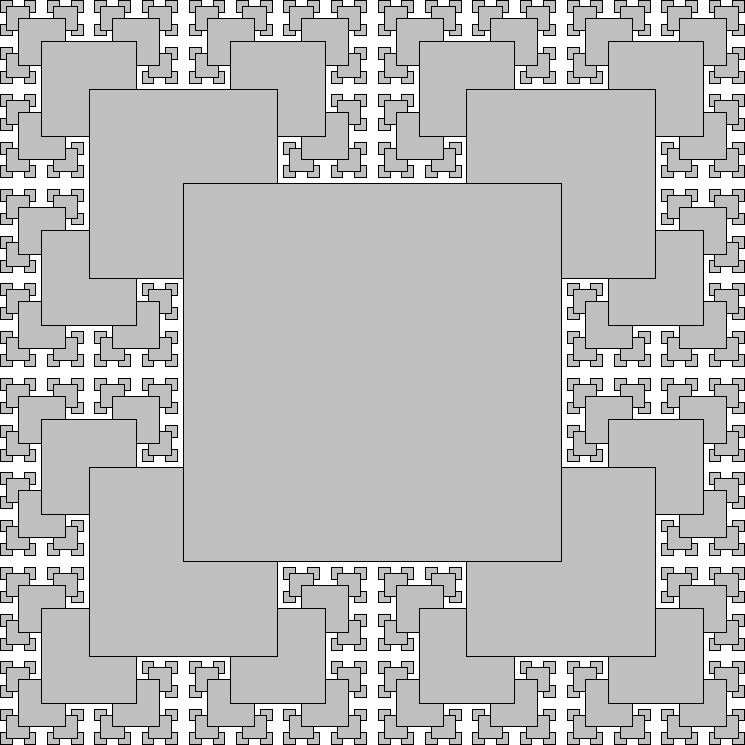
\includegraphics[width=0.8\textwidth]{Figures/FigC.pdf}
	\caption{Fraktál}
	\label{fig:TSquareFractal}
\end{figure}


\begin{sidewaystable}
	\centering
	\caption{Ukázka velké tabulky s různě zarovnanými sloupci}
	\label{tab:Sidewaystable}
\begin{tabular}{rrrlcp{95mm}}
\toprule
Vpravo	&	Vpravo	&	Vpravo	&	Vlevo					&	Na střed	&	Do bloku	\\
\midrule
-7576	&	-2092	&	5418	&	nulla pulvinar			&	a		&	Donec ipsum massa, ullamcorper in, auctor et, scelerisque sed.	\\
-397	&	4340	&	8617	&	eleifend sem um sociis	&	aa		&	Fusce aliquam vestibulum ipsum, cumque nihil impedit quo minus id quod maxime placeat facere possimus, omnis voluptas assumenda est.	\\
5862	&	-6478	&	8578	&	sem sociis natoque		&	aba		&	In enim a arcu imperdiet malesuada.	\\
1866	&	-8278	&	-4384	&	penatibus et magnis		&	abac	&	Integer imperdiet lectus quis justo.	\\
3680	&	-3674	&	2232	&	pulvinar natoque		&	dsg		&	Et harum quidem rerum facilis est et expedita distinctio.	\\
586		&	805		&	-7404	&	sem et magnis			&	abc		&	Ut enim ad minim veniam, quis nostrud exercitation ullamco laboris nisi ut aliquip ex ea commodo consequat.	\\
1388	&	8761	&	-8929	&	sem odio bibendum		&	tsi		&	Phasellus faucibus molestie nisl.	\\
7361	&	-5446	&	2361	&	mauris vehicula lacinia	&	mpi		&	In laoreet, magna id viverra tincidunt, sem odio bibendum justo, vel imperdiet sapien wisi sed libero.	\\
-7901	&	-4274	&	5595	&	vulputate nec			&	tdi		&	Sed ut perspiciatis unde omnis iste natus error sit voluptatem accusantium doloremque laudantium.	\\
-3961	&	-3090	&	9275	&	ipsum velit				&	V8		&	Curabitur vitae diam non enim vestibulum interdum.	\\
\bottomrule
\end{tabular}
\end{sidewaystable}


\begin{sidewaysfigure}
	\centering
	
\includegraphics[width=0.95\textwidth]{Figures/CoffeeAndComputer.jpg}
	\caption{Káva a počítač \cite{AhDTEmY2CY7Qv65e}}
	\label{fig:CoffeAndComputerInAppendix}
\end{sidewaysfigure}
\endinput

% Priloha vlozena primo do hlavniho LaTeX souboru. Ne vsechny prilohy je nutne mit ve zvlastnich souborech.
%\chapter{Dlouhý zdrojový kód}
%\lstinputlisting[label=src:CppExternal,caption={Dlouhý zdrojový kód v jazyce C++ načtený s externího souboru}]{SourceCodes/ArraySortingAlgorithms.cpp}

\end{document}
